\section{Results}
\label{sec:results}


%It has been noticed in the analysis that the central expected values can change by up to $15\%$ when running the full CLs method. 
%The full CLs method, however, takes considerably longer to run, therefore, the full CLs limits did not get ready for the freezing deadline. 

The expected limits shown in this section are obtained with the Higgs Combination tool, with the Asymptotic method. 
Figure~\ref{fig:result_radion} shows the results on spin-0 resonances.
%Figure~\ref{fig:result_graviton} shows the results on spin-2 resonances.  
Figures~\ref{fig:nonres} (in fb) shows the
SM-like non-resonant limit and its breakdown in the different analysis
categories: LM (Low Mass), HM (High Mass), MPC (Medium Purity
Category), and HPC (High Purity Category). 

\begin{figure*}[h]
  \centering
  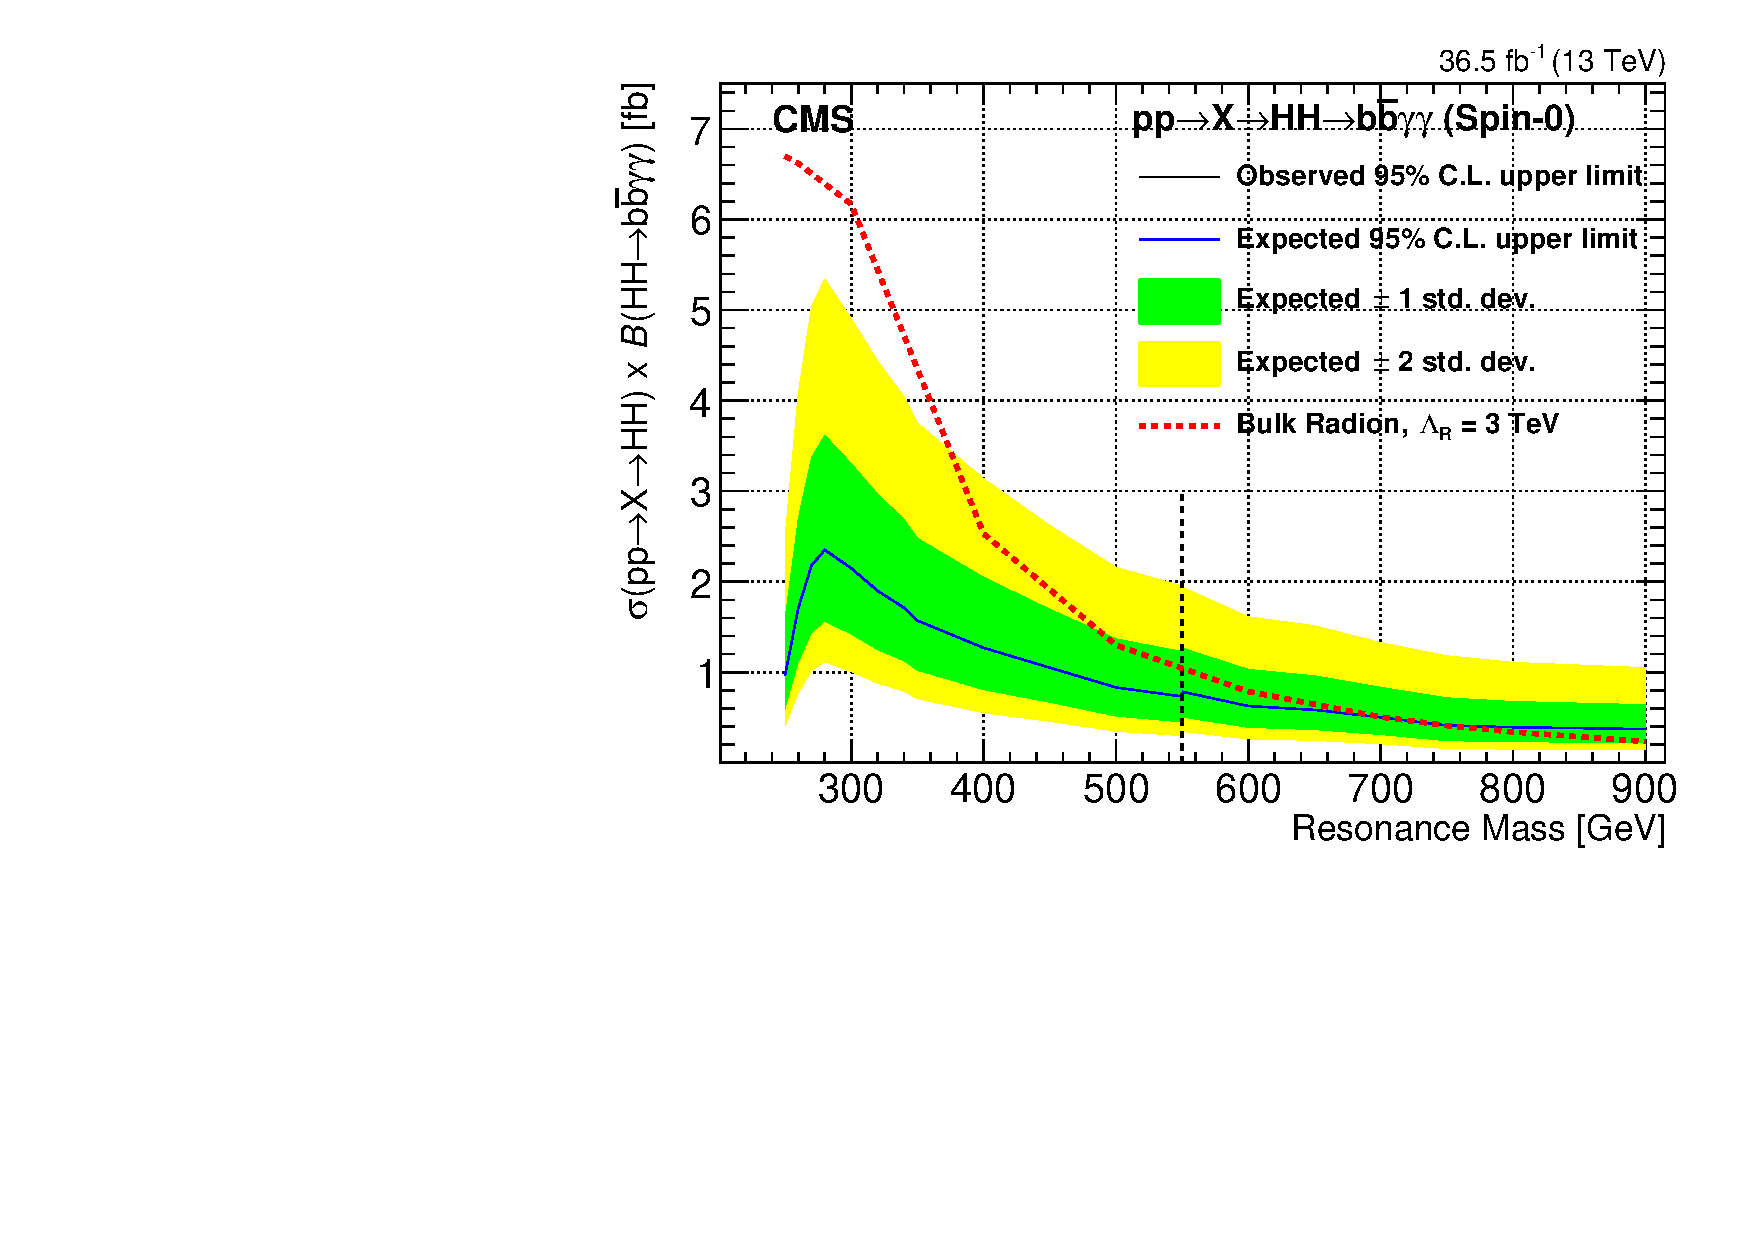
\includegraphics[width=0.65\textwidth]{figures/sec-results/LimsRadionLMHM.pdf}\hfil
  \caption{Limits on spin-0 resonances.}
  \label{fig:result_radion}
\end{figure*}

\begin{figure*}[h]
  \centering
  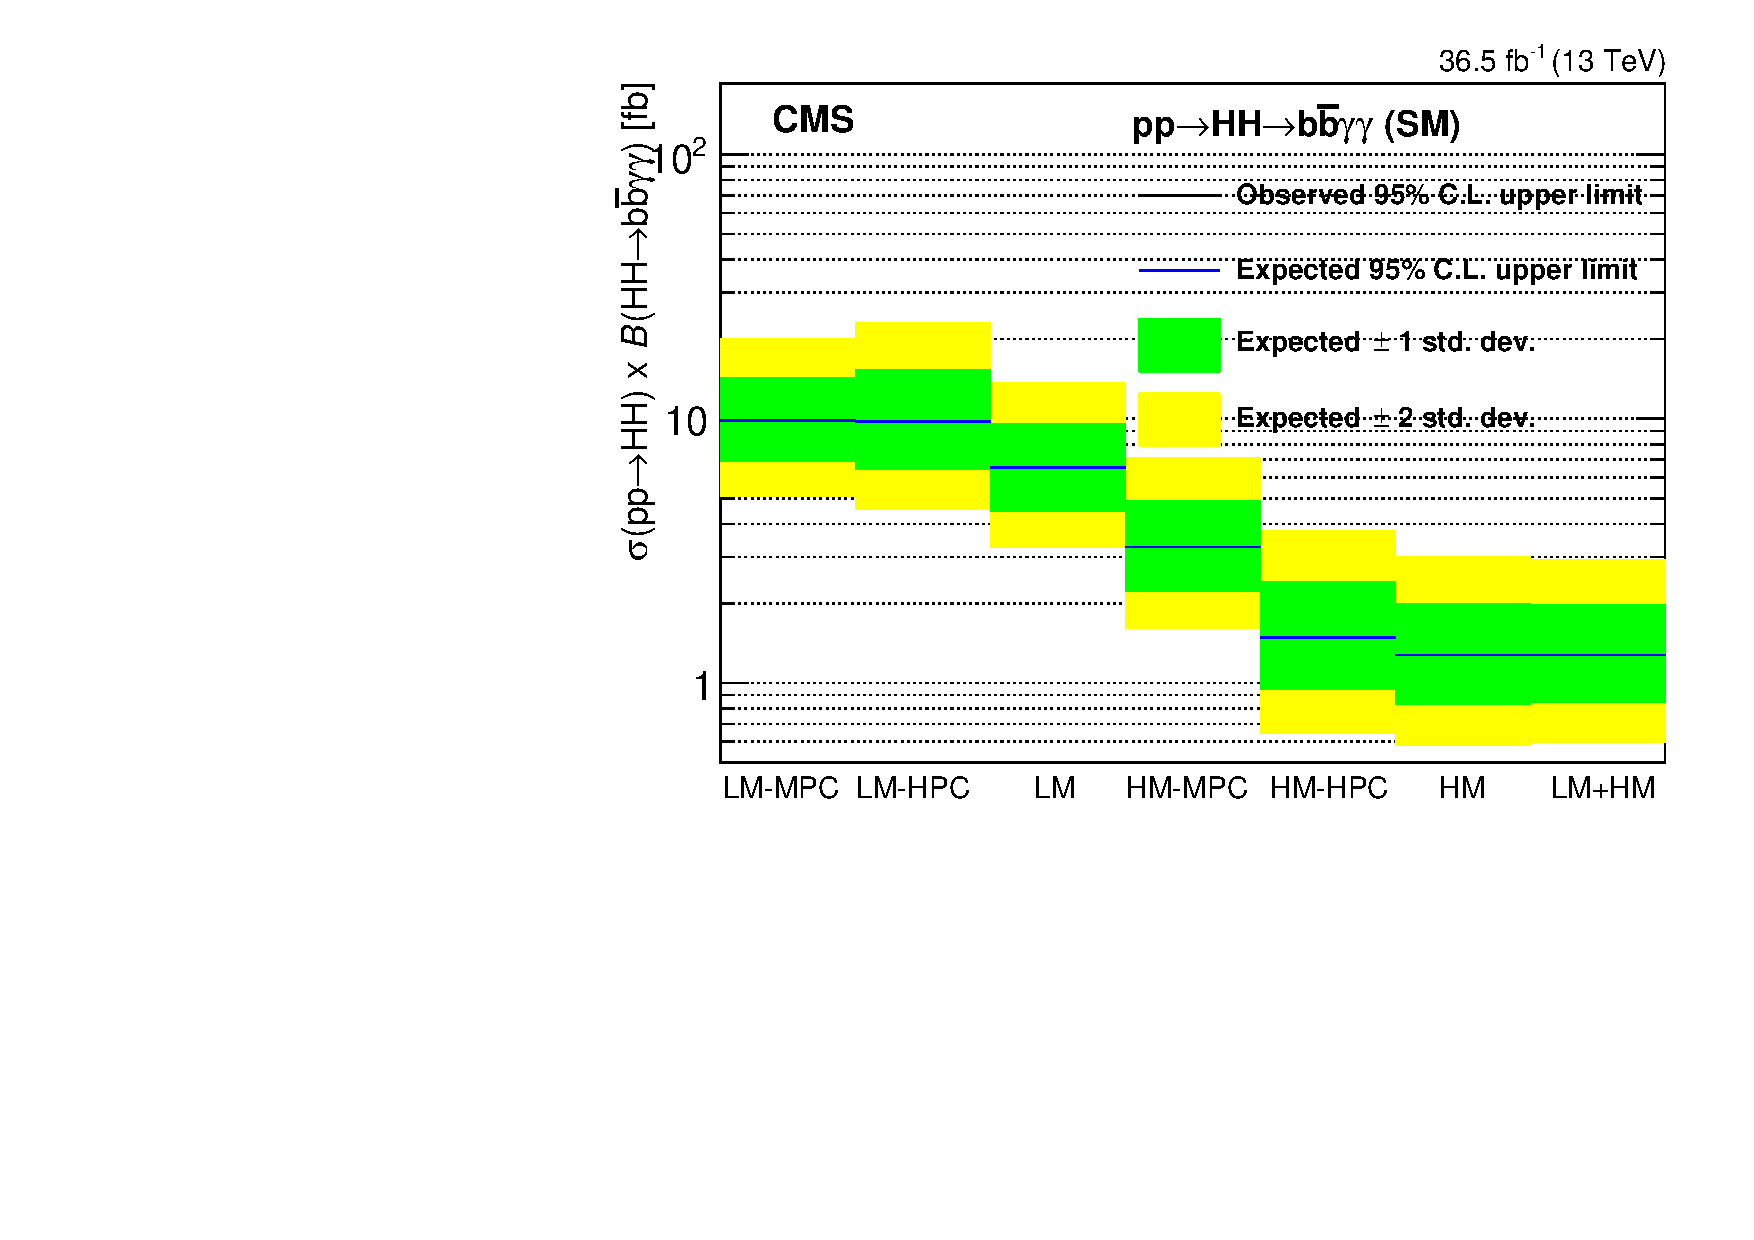
\includegraphics[width=0.65\textwidth]{figures/sec-results/NonResSMCats.pdf}\hfil
  \caption{SM-like non-resonant limits.}
  \label{fig:nonres}
\end{figure*}

As a comparison, expected and observed limits obtained with 2.7 fb$^{-1}$ are shown in Figures \ref{fig:result_radion_2015} and \ref{fig:nonres_2015}. 
The SM-like non-resonant result using 2015 data is a limit about 90 times the SM cross-section.  Scaling this result using a frequentist approach, with the square root of the integrated luminosity ratio of 2.7/35.87, the expected limit with the 2016 dataset is about 25 times the SM cross section. 
The expected limit obtained with the 2016 analysis is, on the other hand, 16.7 times the SM. This represents an improvement on the baseline analysis sensitivity of over $30\%$. 

\begin{figure*}[h]
  \centering
  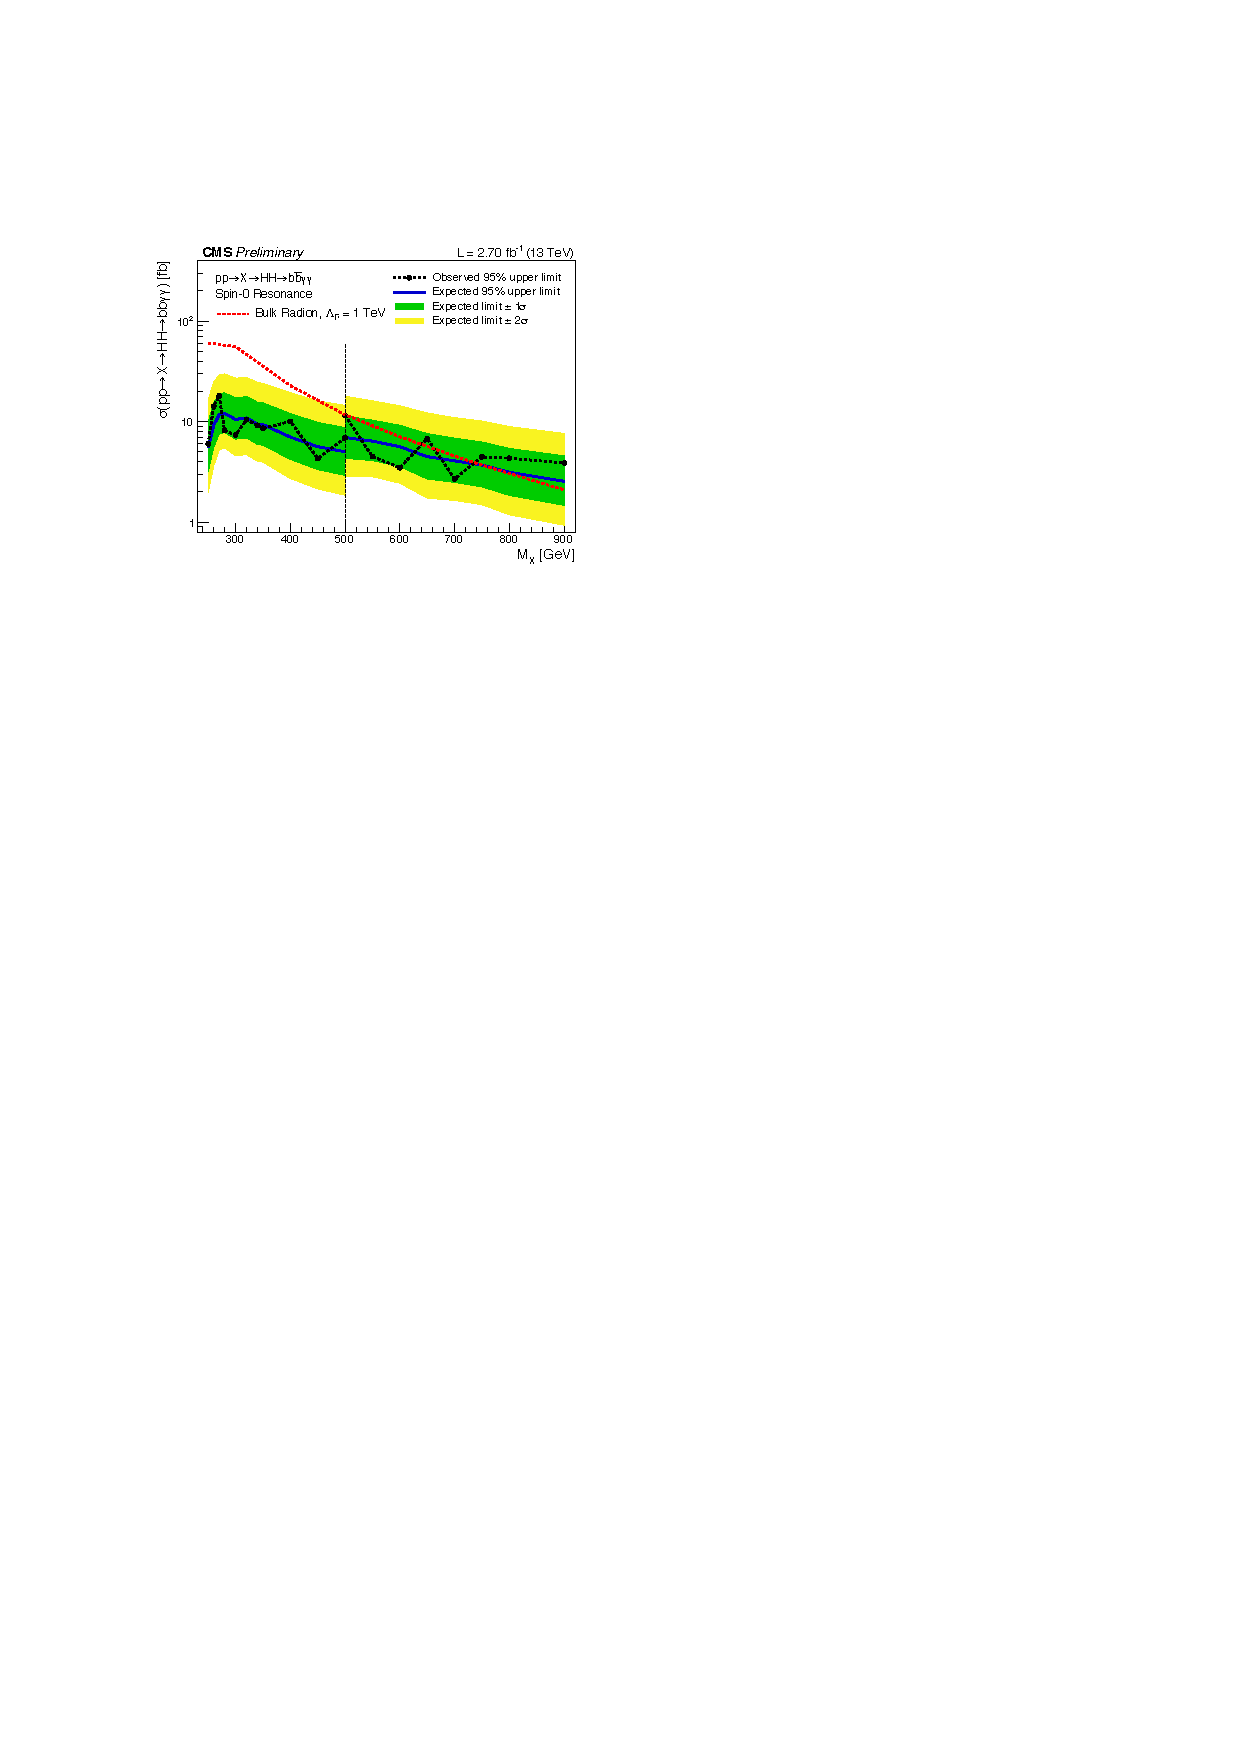
\includegraphics[width=0.65\textwidth]{figures/sec-results/LimsRadionLMHM_2015.pdf}\hfil
  \caption{Limits on spin-0 resonances with the 2015 dataset.}
  \label{fig:result_radion_2015}
\end{figure*}

\begin{figure*}[h]
  \centering
  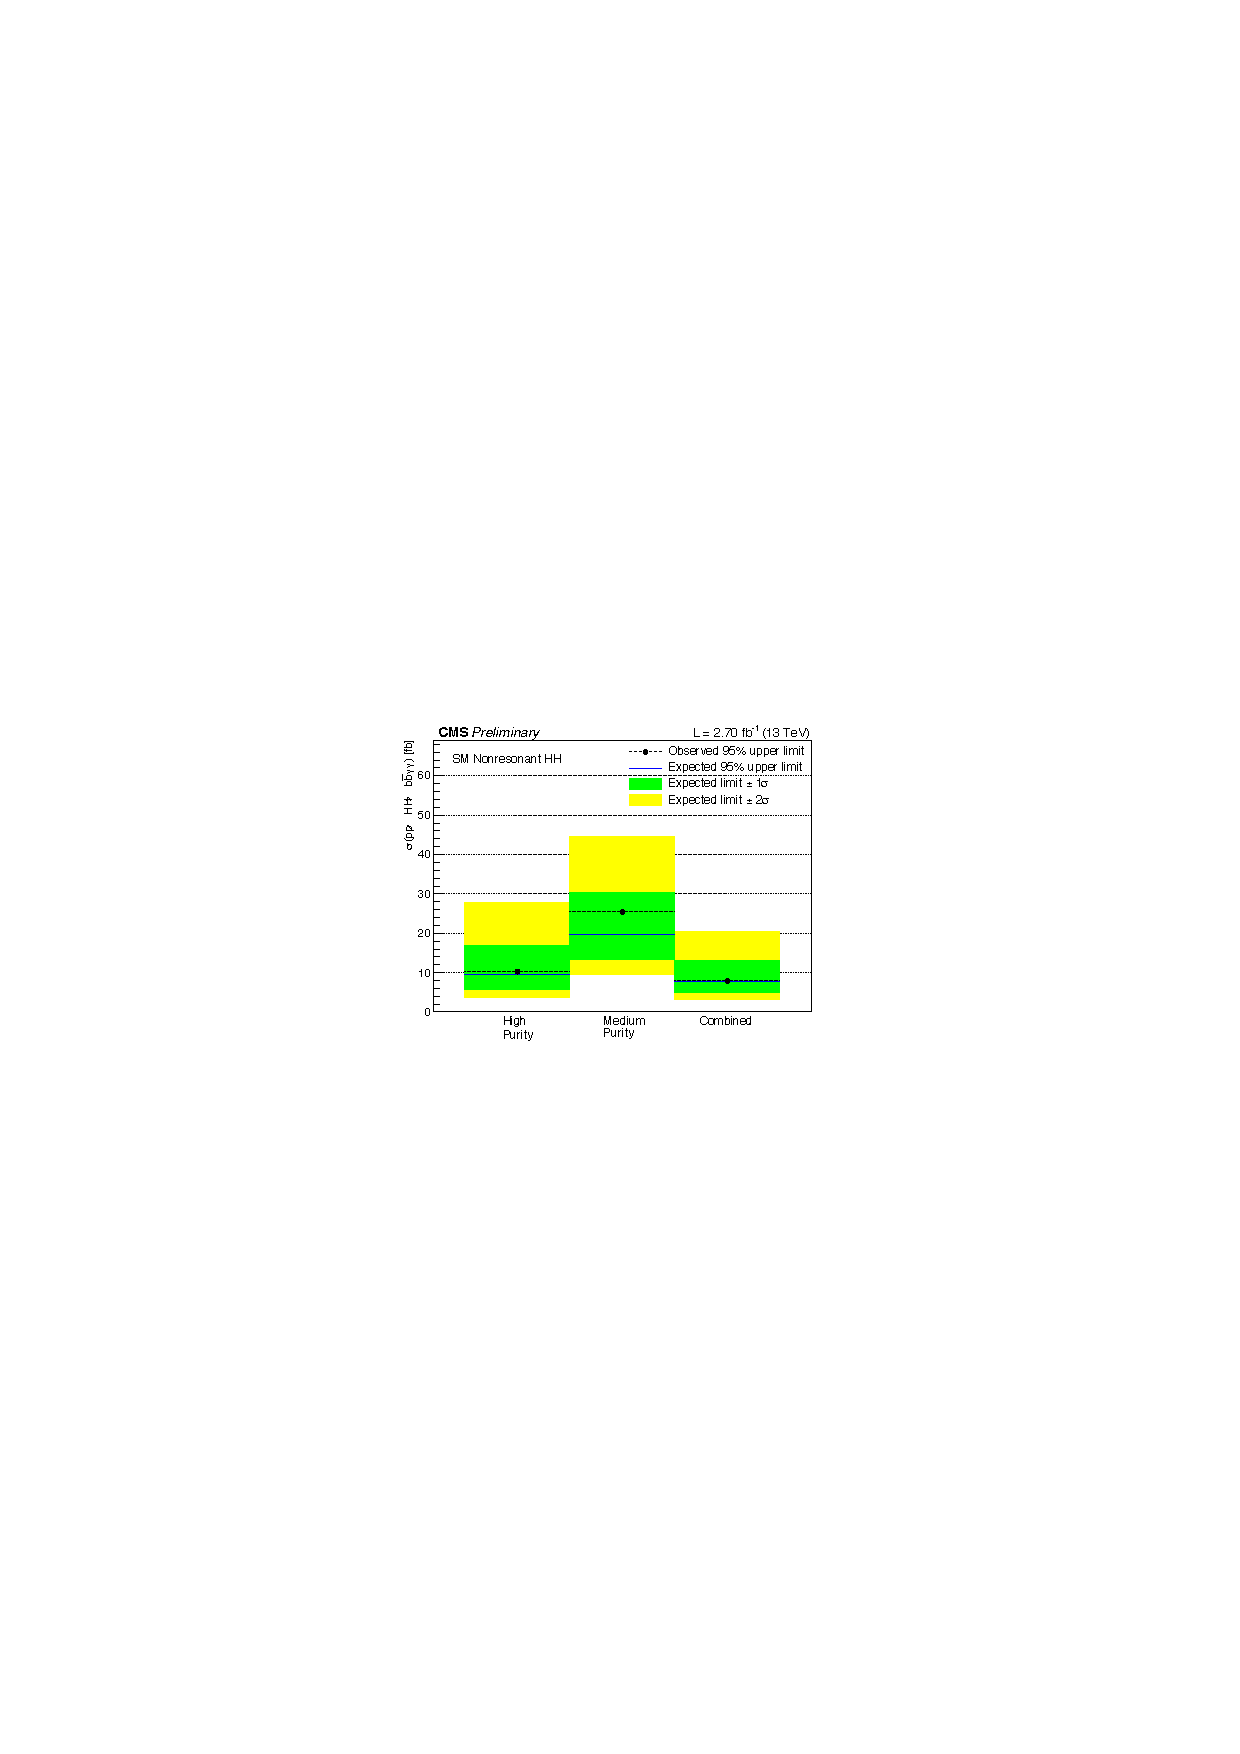
\includegraphics[width=0.65\textwidth]{figures/sec-results/NonResSMCats_2015.pdf}\hfil
  \caption{SM-like non-resonant limits with the 2015 dataset.}
  \label{fig:nonres_2015}
\end{figure*}
